% !TEX program = xelatex
% IA712 - Projet B : Recherche et Sauvetage Autonomes - présentation de 10 minutes (FR)
\documentclass[aspectratio=169,11pt]{beamer}
\usepackage{amsmath}
\usepackage{fontspec}
\usepackage{graphicx}
\graphicspath{{img/}}
\usepackage{tikz}
\usetikzlibrary{arrows.meta,positioning,shapes.geometric,fit,calc}
\usepackage{booktabs}

\definecolor{nccblue}{HTML}{1F4E79}
\definecolor{nccsky}{HTML}{1F6FEB}
\definecolor{nccorange}{HTML}{FB8500}
\definecolor{nccgreen}{HTML}{2DA44E}
\definecolor{nccred}{HTML}{D1242F}
\definecolor{nccdark}{HTML}{222831}

\usetheme{default}
\usecolortheme{default}
\setbeamercolor{structure}{fg=nccblue}
\setbeamercolor{frametitle}{fg=nccblue}
\setbeamertemplate{frametitle}{\vspace{0.6mm}{\color{nccblue}\large\bfseries\insertframetitle}\par\vspace{0.3mm}}
\setbeamertemplate{navigation symbols}{}
\setbeamertemplate{footline}[frame number]
\setbeamerfont{frametitle}{series=\bfseries}
\setbeamertemplate{itemize items}[circle]
\setbeamercolor{itemize item}{fg=nccorange}
\setbeamercolor{itemize subitem}{fg=nccsky}

\tikzset{
  box/.style={rounded corners=2pt,draw=nccblue,fill=nccblue!6,align=center,inner sep=3pt,font=\scriptsize,minimum height=7mm,text width=20mm},
  phase1/.style={box,fill=nccsky!15,draw=nccsky},
  phase2/.style={box,fill=nccorange!15,draw=nccorange},
  io/.style={box,fill=nccgreen!12,draw=nccgreen},
  proc/.style={box,fill=white},
  btnode/.style={box,fill=nccblue!12,draw=nccblue},
  ar/.style={-{Latex[length=2mm]},draw=nccdark!70,semithick},
  arl/.style={ar,font=\tiny,inner sep=1pt},
}

\title{\textbf{Recherche et Sauvetage Autonomes}}
\subtitle{Projet~B - IA712 Robotique Mobile, Projet Final}
\author{\textbf{Équipe RobotZ}\\[3pt]{\footnotesize Julien GIMENEZ \quad Hugo FANCHINI \quad Paul CINTRA \quad Yimou ZHANG}}
\institute{\small \texttt{https://github.com/YiZeems/autonomous-search-and-rescue}}
\date{IA712 - Séance L18}

\begin{document}

% -- Title --
\begin{frame}[plain]
  \titlepage
  \begin{center}\footnotesize
  ROS\,2 Humble $\cdot$ Ignition Gazebo Fortress $\cdot$ TurtleBot~4 $\cdot$ Nav2 $\cdot$ slam\_toolbox $\cdot$ BehaviorTree.CPP
  \end{center}
\end{frame}

% -- Problem --
\begin{frame}{La mission : recherche \& sauvetage autonomes}
  \begin{columns}[T]
  \begin{column}{0.58\linewidth}
  \textbf{Scénario :} un robot explore une zone sinistrée inconnue, trouve des « victimes » (AprilTags),
  et rapporte leurs coordonnées dans le repère global - \emph{sans intervention humaine}.
  \smallskip
  \textbf{Exigences que nous satisfaisons :}
  {\small\begin{itemize}
    \item Exploration par frontières autonome, carte $>90\,\%$
    \item Détection caméra vers \texttt{map} via \texttt{tf2}
    \item Qualité de carte / fermeture de boucle (SLAM)
    \item \textbf{Décision = Arbre de Comportement, pas FSM}
    \item Lancement en un clic
    \item Bonus : glouton vs.\ gain d'information
  \end{itemize}}
  \end{column}
  \begin{column}{0.40\linewidth}
  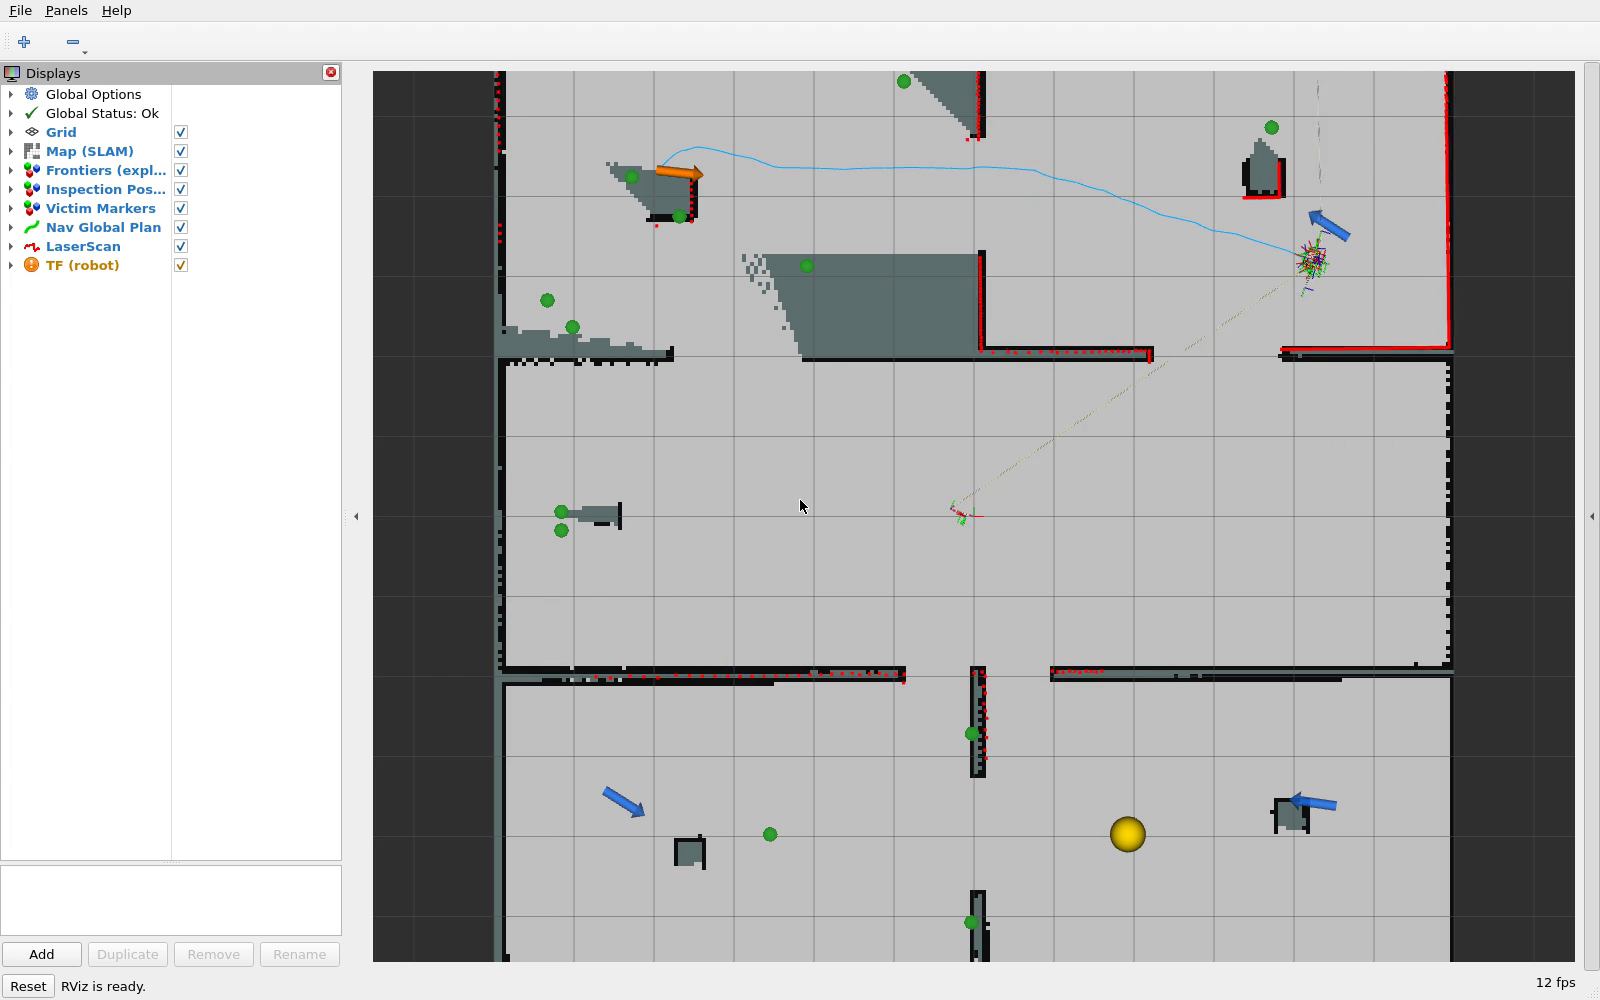
\includegraphics[width=\linewidth]{rviz_live}\\
  {\scriptsize RViz en direct : carte + 4 victimes + algorithmes.}
  \end{column}
  \end{columns}
  \vfill
  {\footnotesize\color{nccblue}\textbf{Résultat :} un run autonome continu - \textbf{97,35\,\% de couverture, 4/4 victimes}.}
\end{frame}

% -- Architecture --
\begin{frame}{Architecture du système - quatre paquets ROS\,2}
  \centering
  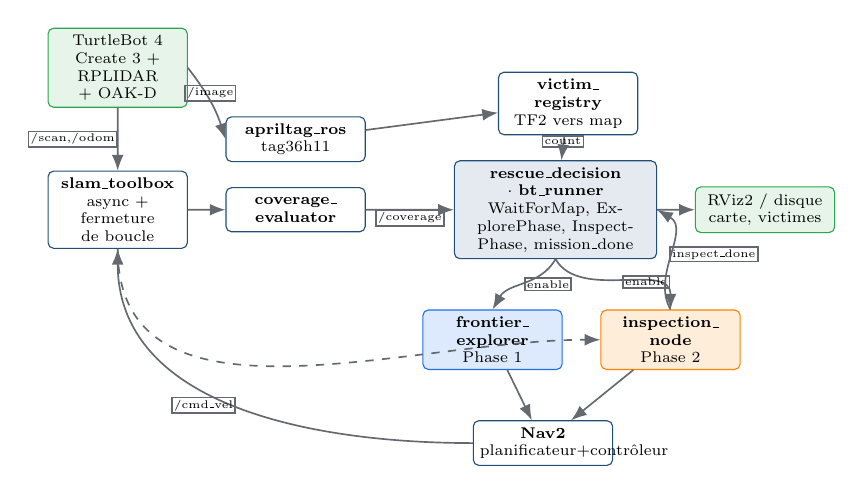
\begin{tikzpicture}[node distance=4mm and 6mm,scale=0.8,transform shape]
    \node[io] (robot) {TurtleBot~4\\\scriptsize Create~3 + RPLIDAR + OAK-D};
    \node[proc,below=10mm of robot] (slam) {\textbf{slam\_toolbox}\\\scriptsize async + fermeture de boucle};
    \node[proc,right=of slam] (metric) {\textbf{coverage\_}\\\textbf{evaluator}};
    \node[proc,above=of metric] (april) {\textbf{apriltag\_ros}\\\scriptsize tag36h11};
    \node[btnode,right=14mm of metric,text width=30mm] (bt) {\textbf{rescue\_decision $\cdot$ bt\_runner}\\\scriptsize WaitForMap, ExplorePhase, InspectPhase, mission\_done};
    \node[phase1,below=8mm of bt,xshift=-10mm] (explore) {\textbf{frontier\_}\\\textbf{explorer}\\\scriptsize Phase 1};
    \node[phase2,right=of explore] (inspect) {\textbf{inspection\_}\\\textbf{node}\\\scriptsize Phase 2};
    \node[proc,below=8mm of explore,xshift=8mm] (nav) {\textbf{Nav2}\\\scriptsize planificateur+contrôleur};
    \node[proc,above=of bt,xshift=2mm] (reg) {\textbf{victim\_}\\\textbf{registry}\\\scriptsize TF2 vers map};
    \node[io,right=of bt] (rviz) {RViz2 / disque\\\scriptsize carte, victimes};
    \draw[ar] (robot) -- node[arl,left]{/scan,/odom} (slam);
    \draw[ar] (robot.east) to[bend left=10] node[arl,above]{/image} (april.west);
    \draw[ar] (slam) -- (metric);
    \draw[ar] (april) -- (reg);
    \draw[ar] (metric) -- node[arl,below]{/coverage} (bt);
    \draw[ar] (bt.south) to[out=-120,in=60] node[arl,right]{enable} (explore.north);
    \draw[ar] (bt.south) to[out=-60,in=90] node[arl,right]{enable} (inspect.north);
    \draw[ar] (inspect.north) to[out=120,in=-30] node[arl,right]{inspect\_done} (bt.east);
    \draw[ar] (explore) -- (nav);
    \draw[ar] (inspect) -- (nav);
    \draw[ar] (nav.west) to[out=180,in=-90] node[arl,left]{/cmd\_vel} (slam.south);
    \draw[ar] (reg) -- node[arl,above]{count} (bt);
    \draw[ar] (bt) -- (rviz);
    \draw[ar,dashed] (slam) to[out=-90,in=180] (inspect.west);
  \end{tikzpicture}
  \par\smallskip
  {\footnotesize L'\textbf{Arbre de Comportement orchestre} : il cadence l'explorateur (Phase 1) et l'inspecteur
  (Phase 2) via les topics \texttt{/mission/*} ; les nœuds Python font le travail. Le SLAM alimente la carte
  vers l'exploration, la couverture, Nav2 et l'inspection.}
\end{frame}

% -- Two-phase BT --
\begin{frame}{Mission en deux phases orchestrée par l'Arbre de Comportement}
  \begin{columns}[T]
  \begin{column}{0.36\linewidth}
  \centering
  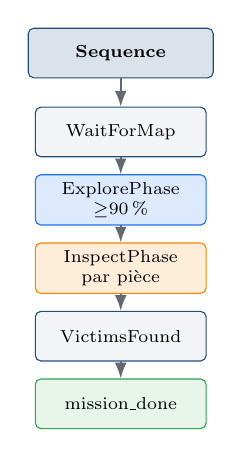
\begin{tikzpicture}[node distance=2.4mm,scale=0.9,transform shape]
    \node[box,fill=nccblue!16,text width=24mm] (root){\textbf{Sequence}};
    \node[box,below=4mm of root,text width=22mm](n1){WaitForMap};
    \node[phase1,below=of n1,text width=22mm](n2){ExplorePhase\\\scriptsize $\geq$90\,\%};
    \node[phase2,below=of n2,text width=22mm](n3){InspectPhase\\\scriptsize par pièce};
    \node[box,below=of n3,text width=22mm](n4){VictimsFound};
    \node[io,below=of n4,text width=22mm](n5){mission\_done};
    \draw[ar](root)--(n1);\draw[ar](n1)--(n2);\draw[ar](n2)--(n3);\draw[ar](n3)--(n4);\draw[ar](n4)--(n5);
  \end{tikzpicture}
  \end{column}
  \begin{column}{0.62\linewidth}
  
\includegraphics[width=\linewidth]{algorithms_two_phase}\\
  {\scriptsize \textbf{Phase 1} (bleu) l'exploration par frontières construit la carte ; \textbf{Phase 2} (orange)
  inspecte chaque pièce à des poses \emph{dérivées de la carte} (sans coordonnées des victimes) pour capter chaque tag mural.}
  \end{column}
  \end{columns}
  \smallskip
  {\footnotesize\color{nccblue} Pourquoi deux phases ? L'exploration pure cartographie les pièces depuis les portes mais la caméra
  ne s'approche jamais à moins de 2\,m des tags muraux, donc elle plafonne à $\sim$2 victimes.}
\end{frame}

% -- Concepts --
\begin{frame}{Fondements théoriques}
  \begin{columns}[T]
  \begin{column}{0.54\linewidth}
  {\small\begin{itemize}
    \item \textbf{SLAM + fermeture de boucle} - carte en ligne cohérente.
    \item \textbf{Exploration par frontières} - limite libre/inconnu ; \emph{gain d'information}
      $g(f)=\text{gain}-\lambda\,\text{coût}$. Liste noire des frontières mortes (échec Nav2, ou 3$\times$ sans gain, écartée).
    \item \textbf{Planification de chemin} - Dijkstra/NavFn vs.\ A* ; NavFn conservé (tolérant en espace étroit).
    \item \textbf{TF2} - projection détection caméra vers le repère global \texttt{map} (exigence du projet).
    \item \textbf{Arbre de Comportement} - réactif, composable ; \texttt{Sequence} à mémoire, pas une FSM.
  \end{itemize}}
  \end{column}
  \begin{column}{0.44\linewidth}
  \centering
  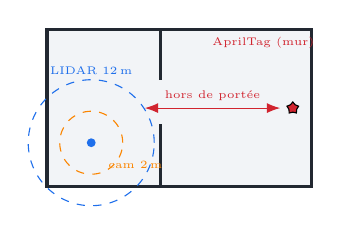
\begin{tikzpicture}[font=\scriptsize,scale=0.80,transform shape]
    \fill[nccblue!6] (0,0) rectangle (4.2,2.5); \draw[very thick,nccdark] (0,0) rectangle (4.2,2.5);
    \draw[very thick,nccdark] (1.8,2.5)--(1.8,1.7);\draw[very thick,nccdark] (1.8,0)--(1.8,1.0);
    \node[star,star points=5,fill=nccred,draw=black,inner sep=1.3pt] at (3.9,1.25){};
    \node[nccred,right] at (2.5,2.28){\tiny AprilTag (mur)};
    \fill[nccsky] (0.7,0.7) circle (2pt);
    \draw[dashed,nccsky] (0.7,0.7) circle (1.0cm);\node[nccsky] at (0.7,1.85){\tiny LIDAR 12\,m};
    \draw[dashed,nccorange](0.7,0.7) circle (0.5cm);\node[nccorange] at (1.4,0.35){\tiny cam 2\,m};
    \draw[{Latex}-{Latex},nccred](1.55,1.25)--(3.7,1.25)node[midway,above]{\tiny hors de portée};
  \end{tikzpicture}\\
  {\scriptsize L'écart caméra-vs-LIDAR que la phase d'inspection comble.}
  \end{column}
  \end{columns}
\end{frame}

% -- Journey --
\begin{frame}{Le parcours de décision - trois runs}
  \centering
  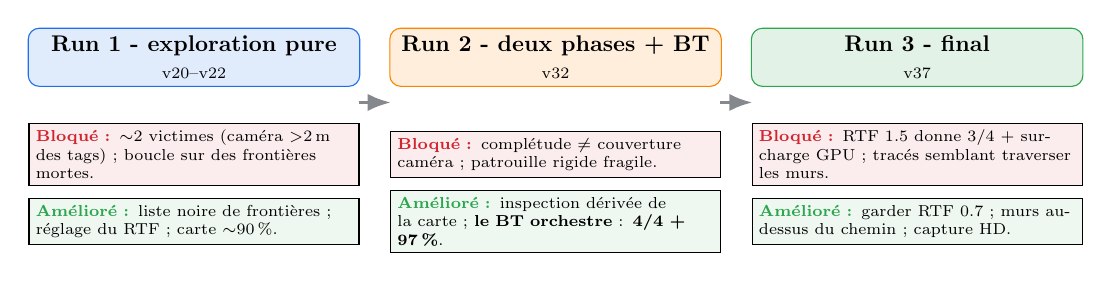
\begin{tikzpicture}[font=\scriptsize,scale=0.82,transform shape]
  \foreach \i/\x/\c/\t/\v in {1/0/nccsky/{Run 1 - exploration pure}/{v20–v22},2/5.6/nccorange/{Run 2 - deux phases + BT}/{v32},3/11.2/nccgreen/{Run 3 - final}/{v37}}{
    \node[draw=\c,fill=\c!14,rounded corners,text width=4.9cm,align=center,font=\bfseries,minimum height=7mm](h\i) at (\x+2.45,4.4){\t\\\normalfont\scriptsize \v};}
  \node[draw,fill=nccred!8,text width=4.9cm,align=left,inner sep=3pt](b1) at (2.45,2.9){\textbf{\color{nccred}Bloqué :} $\sim$2 victimes (caméra $>$2\,m des tags) ; boucle sur des frontières mortes.};
  \node[draw,fill=nccgreen!8,text width=4.9cm,align=left,inner sep=3pt,below=2mm of b1](i1){\textbf{\color{nccgreen}Amélioré :} liste noire de frontières ; réglage du RTF ; carte $\sim$90\,\%.};
  \node[draw,fill=nccred!8,text width=4.9cm,align=left,inner sep=3pt](b2) at (8.05,2.9){\textbf{\color{nccred}Bloqué :} complétude $\neq$ couverture caméra ; patrouille rigide fragile.};
  \node[draw,fill=nccgreen!8,text width=4.9cm,align=left,inner sep=3pt,below=2mm of b2](i2){\textbf{\color{nccgreen}Amélioré :} inspection dérivée de la carte ; \textbf{le BT orchestre} : \textbf{4/4 + 97\,\%}.};
  \node[draw,fill=nccred!8,text width=4.9cm,align=left,inner sep=3pt](b3) at (13.65,2.9){\textbf{\color{nccred}Bloqué :} RTF~1.5 donne 3/4 + surcharge GPU ; tracés semblant traverser les murs.};
  \node[draw,fill=nccgreen!8,text width=4.9cm,align=left,inner sep=3pt,below=2mm of b3](i3){\textbf{\color{nccgreen}Amélioré :} garder RTF~0.7 ; murs au-dessus du chemin ; capture HD.};
  \draw[-{Latex},very thick,nccdark!55] (5.0,3.7)--(5.5,3.7);
  \draw[-{Latex},very thick,nccdark!55] (10.6,3.7)--(11.1,3.7);
  \end{tikzpicture}
  \par\smallskip
  {\footnotesize Deux causes racines cachées : le coût Nav2 décourageait l'\emph{entrée} dans les pièces (couverture) ; un
  RTF effondré \emph{affamait la caméra} (détection). Le BT à 2 phases a ensuite rendu le 4/4 fiable.}
\end{frame}

% -- Results 1 --
\begin{frame}{Résultats - algorithmes en direct dans RViz}
  \centering
  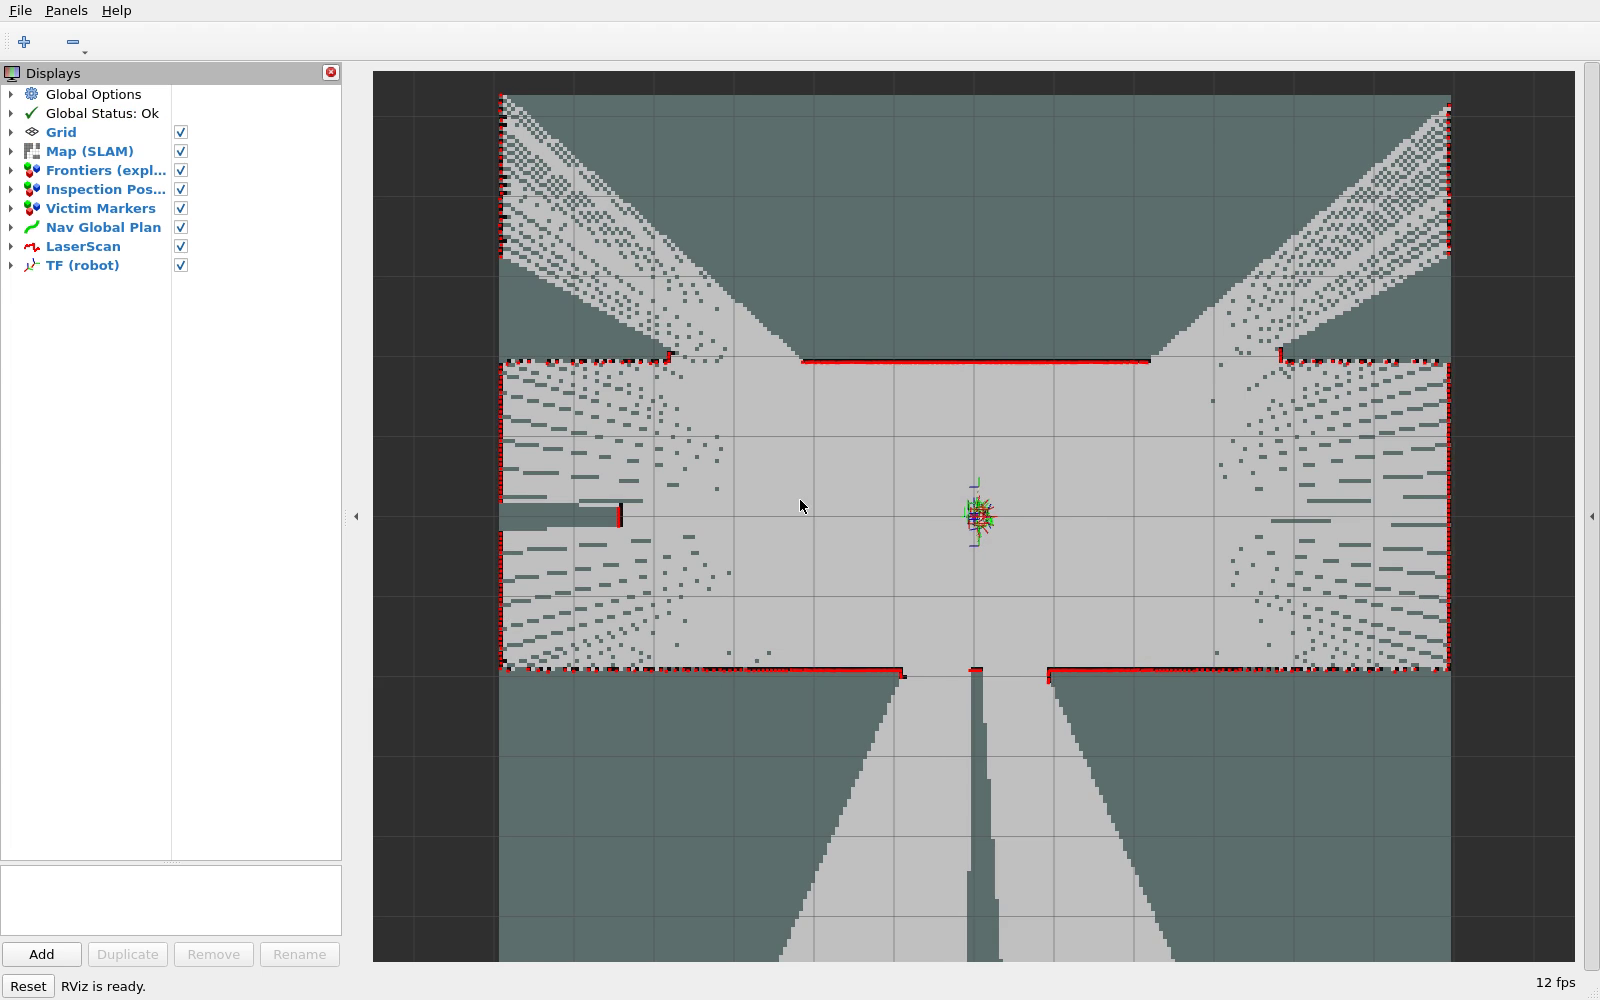
\includegraphics[width=0.275\linewidth]{rviz_seq_1}\hfill
  
\includegraphics[width=0.275\linewidth]{rviz_seq_3}\hfill
  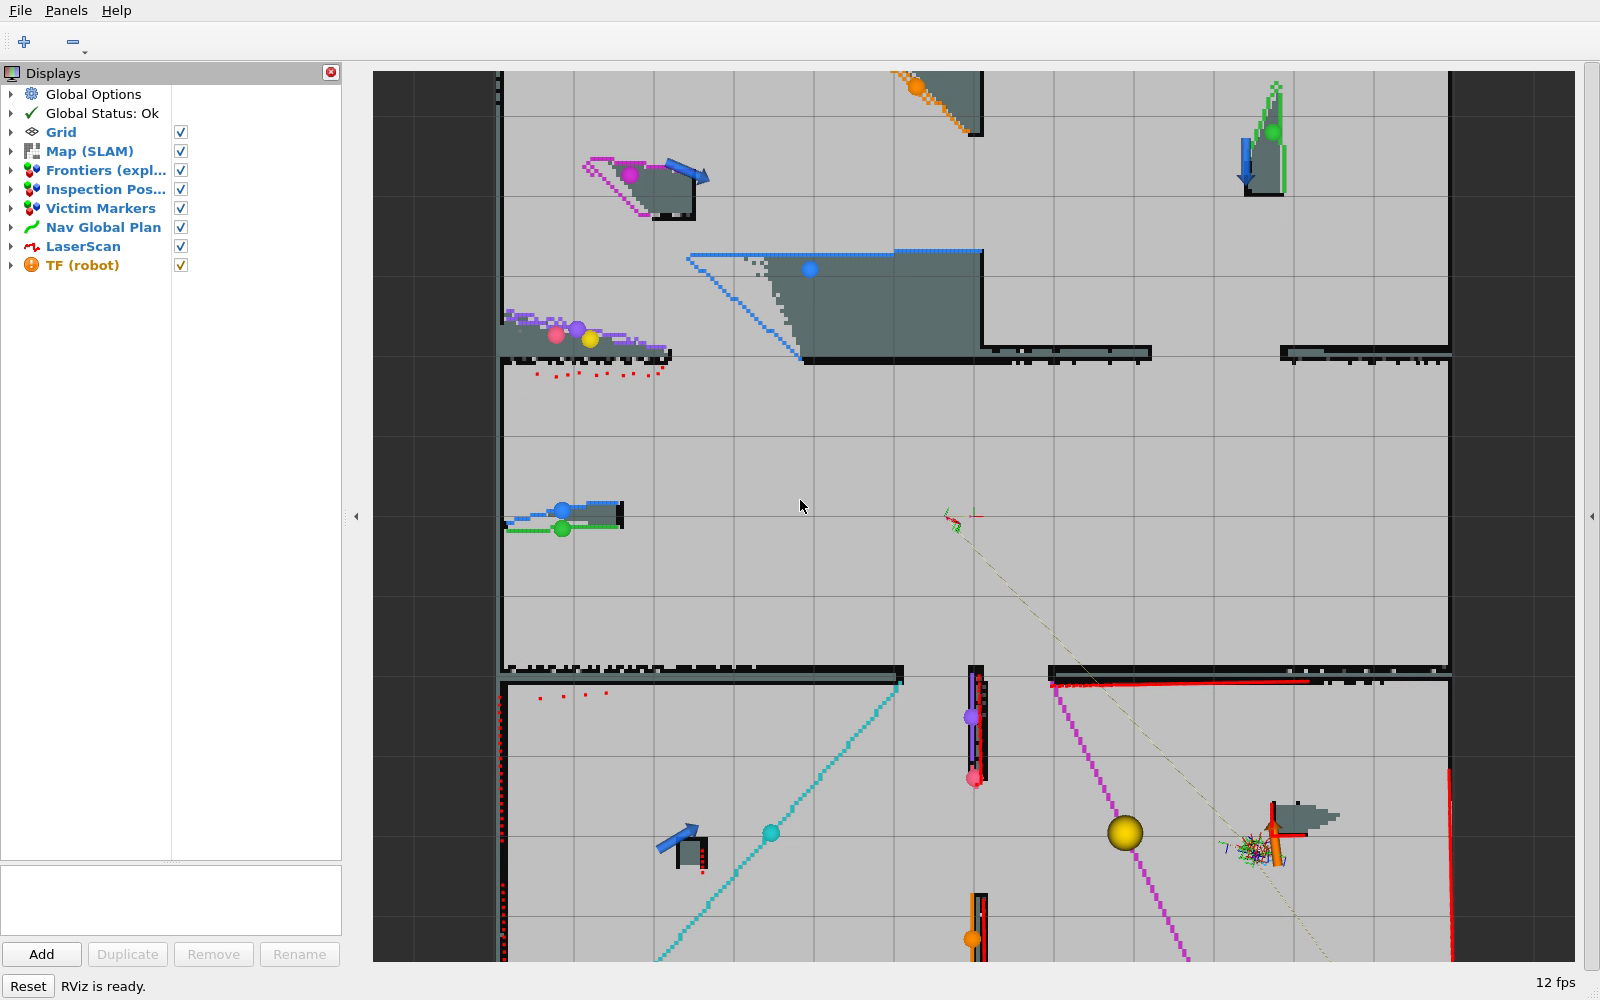
\includegraphics[width=0.275\linewidth]{rviz_seq_4}\\[1pt]
  
\includegraphics[width=0.275\linewidth]{rviz_seq_5}\hfill
  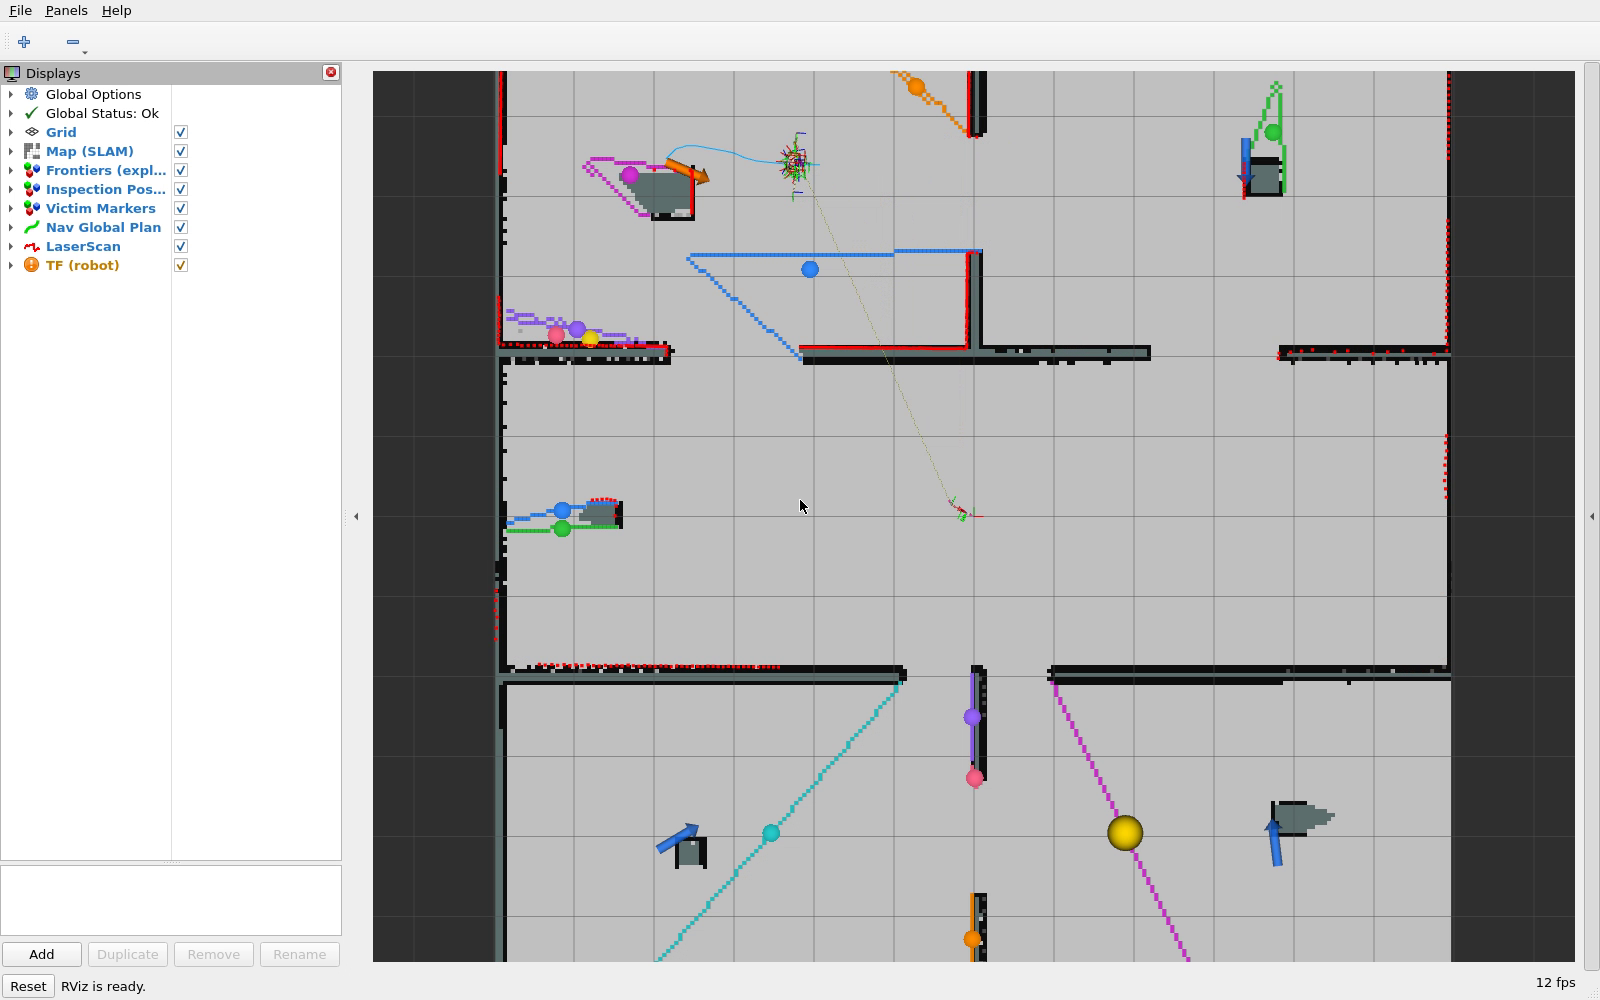
\includegraphics[width=0.275\linewidth]{rviz_seq_6}\hfill
  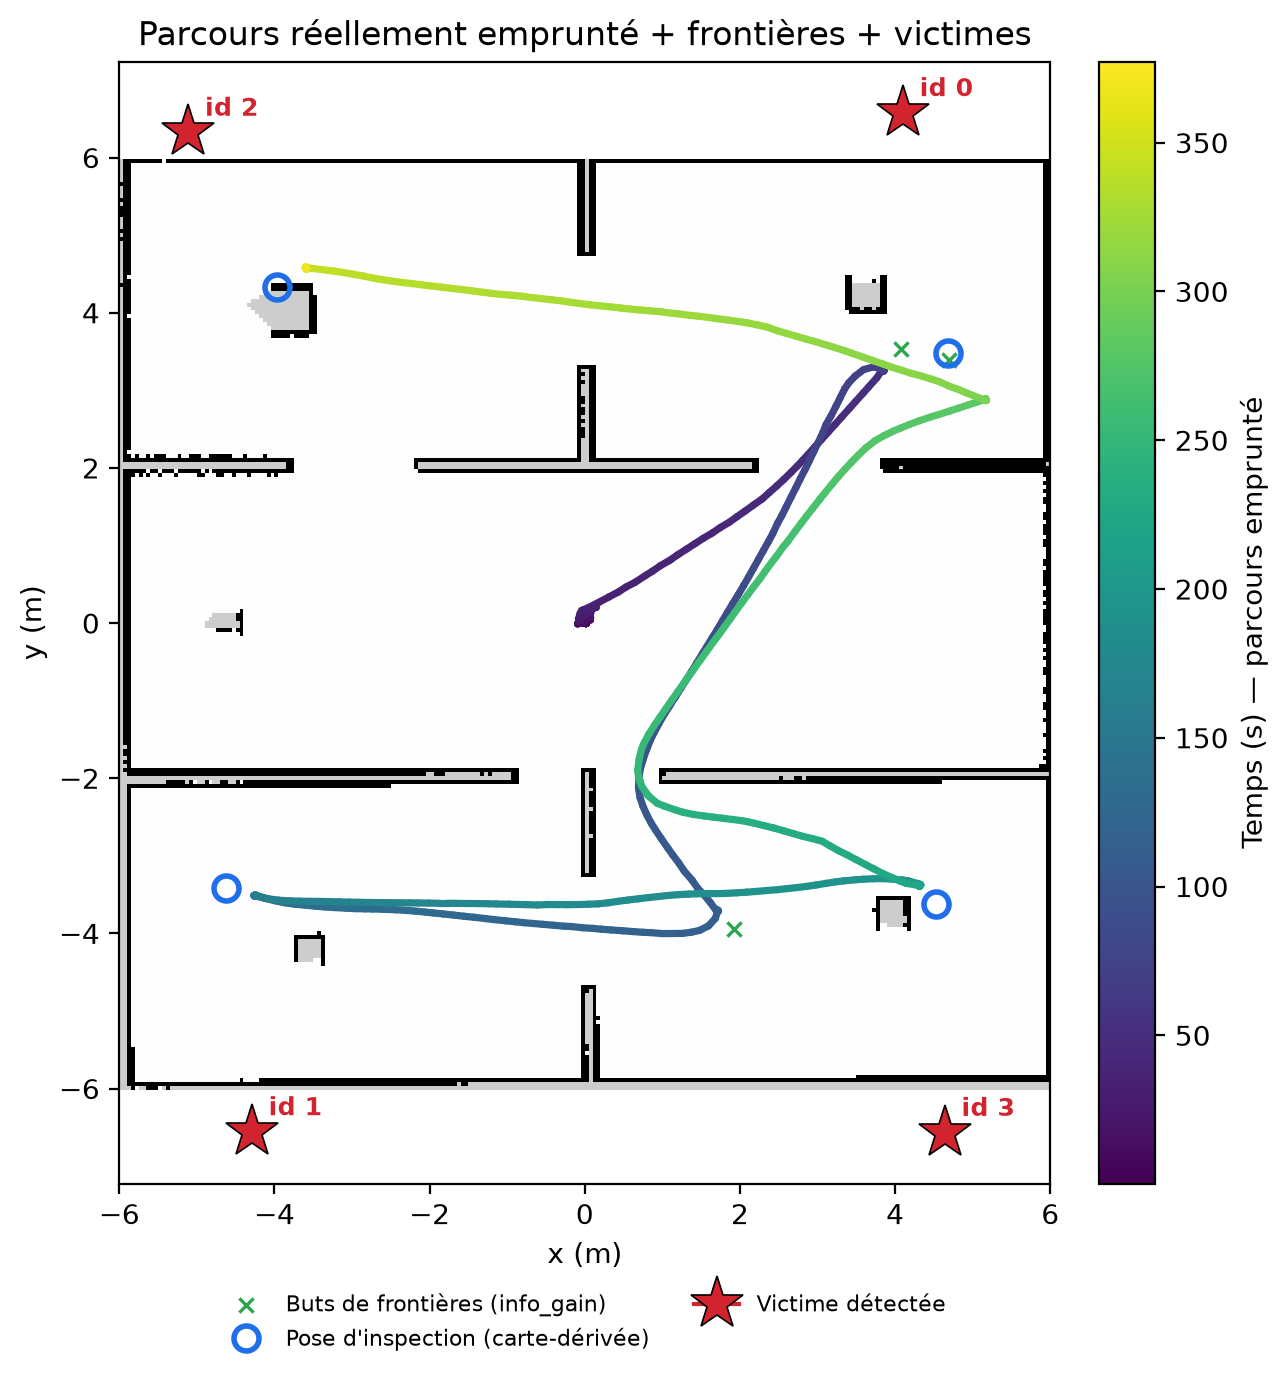
\includegraphics[width=0.275\linewidth]{trajectory_map}
  \par\smallskip
  {\scriptsize Exploration, inspection, quatre victimes ; en bas à droite : le chemin réel
  (repère carte, murs tracés par-dessus - il enfile les portes, aucun segment ne traverse un mur).}
\end{frame}

% -- Voir l'algorithme : Gazebo vs RViz frontieres --
\begin{frame}{Voir l'algorithme : Gazebo vs RViz}
  \begin{columns}[c]
  \begin{column}{0.5\linewidth}\centering
  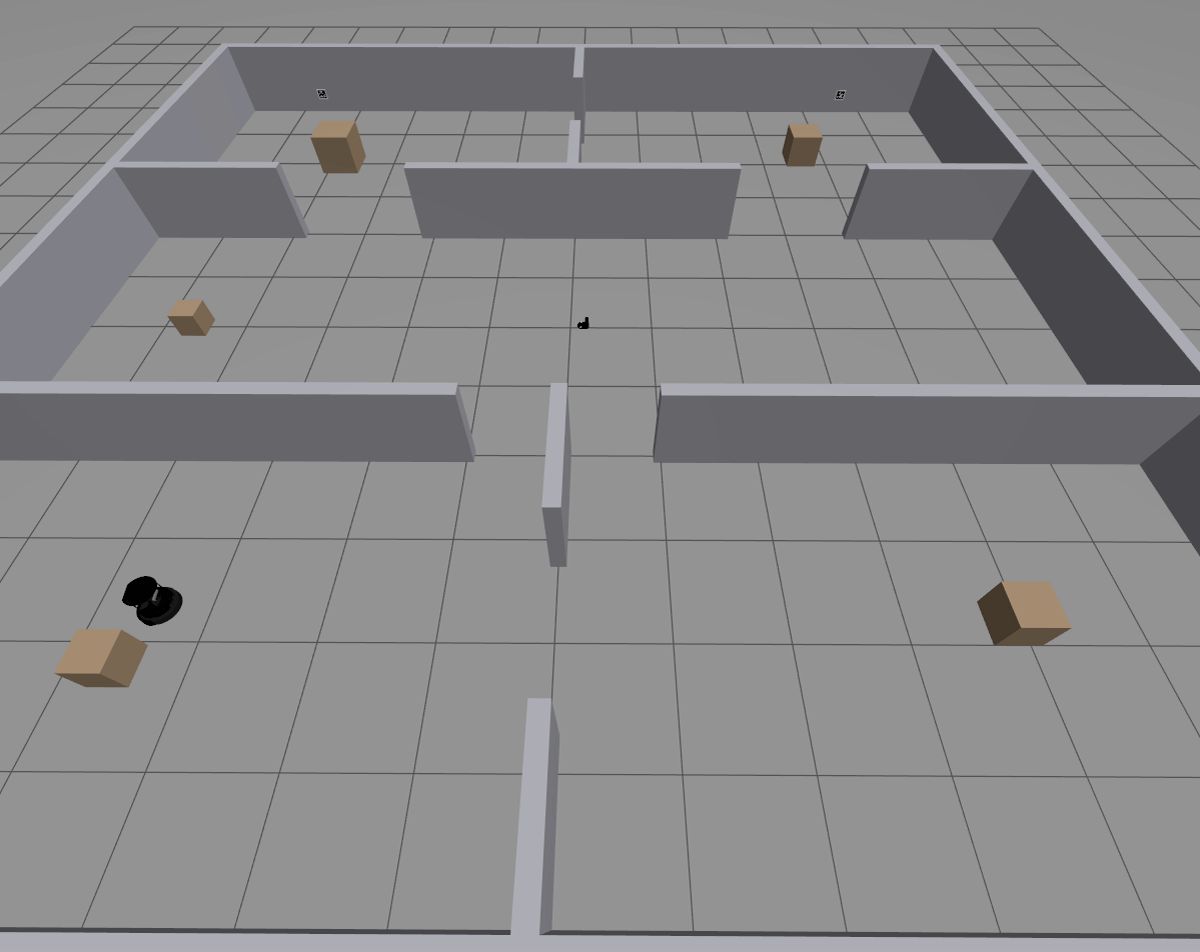
\includegraphics[width=0.90\linewidth]{gazebo_arena}\\[2pt]
  {\scriptsize \textbf{Gazebo} - l'arène simulée : murs, victimes (AprilTags) et le robot.}
  \end{column}
  \begin{column}{0.5\linewidth}\centering
  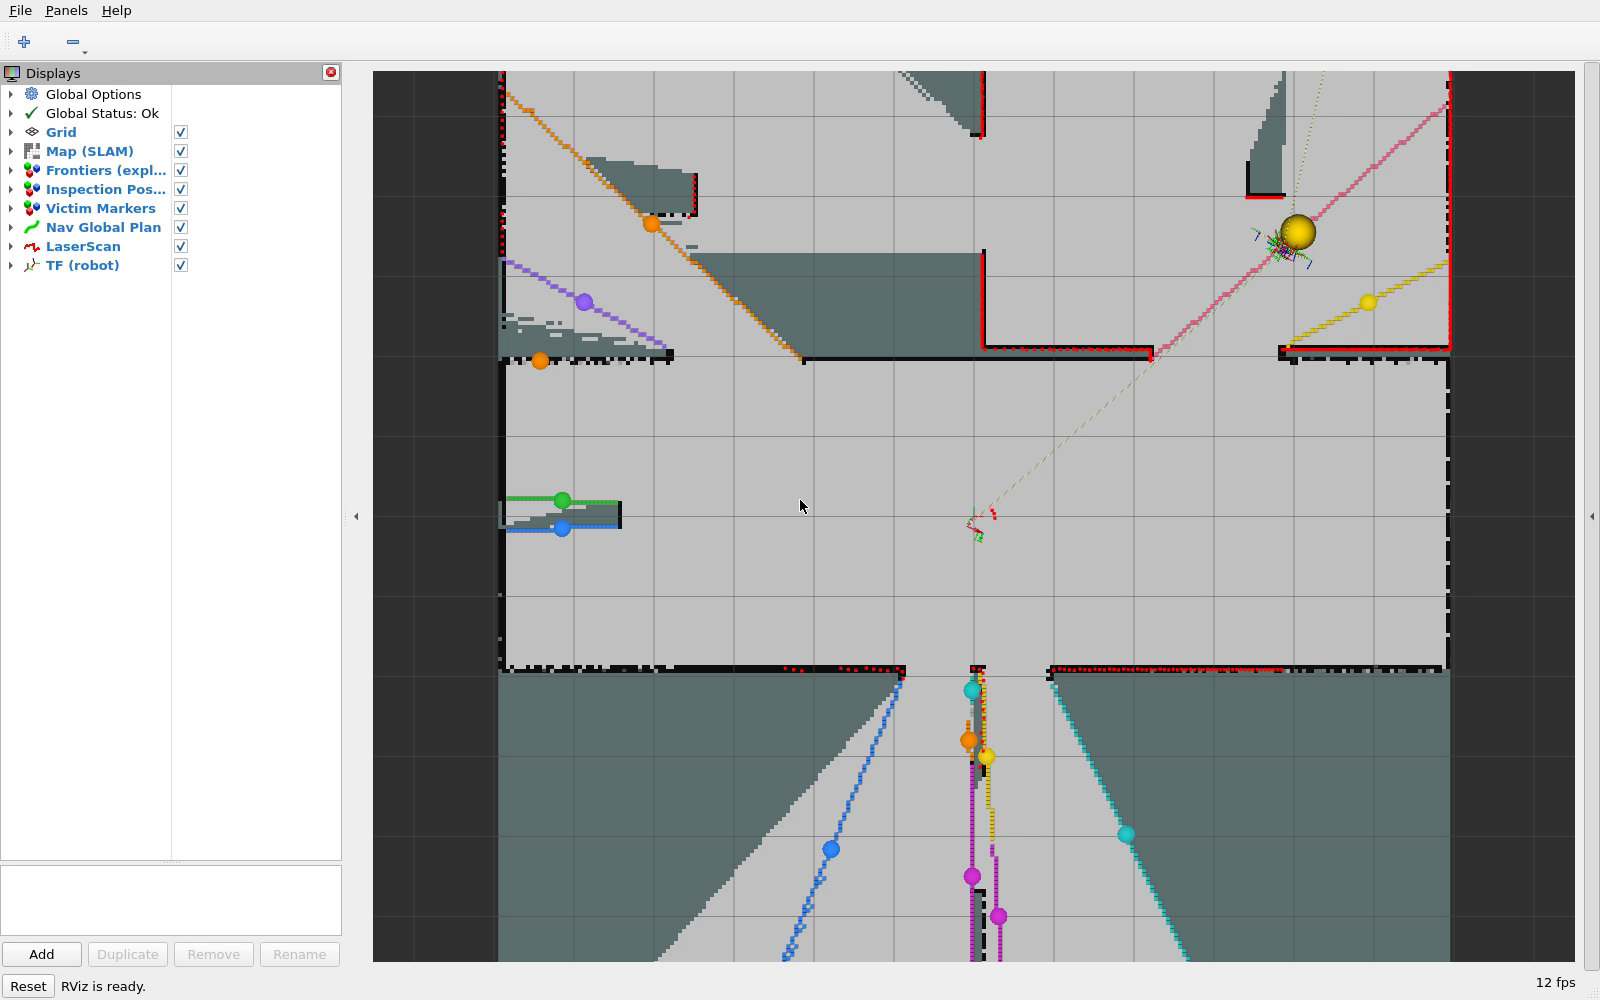
\includegraphics[width=0.90\linewidth]{rviz_frontiers}\\[2pt]
  {\scriptsize \textbf{RViz} - la carte SLAM + les \emph{cellules de frontière colorées par cluster}, la frontière-but (jaune) et le plan Nav2 (bleu).}
  \end{column}
  \end{columns}
  \smallskip
  {\footnotesize\color{nccblue}\centering Chaque \emph{cluster} de frontières a sa couleur, le robot vise la meilleure utilité $g=\text{gain}-\lambda\,\text{coût}$, et l'on \emph{voit} le liseré grignoter l'inconnu jusqu'à $>90\,\%$. Captures : \texttt{gazebo\_capture.mp4} \& \texttt{rviz\_capture.mp4}.}
\end{frame}

% -- Démonstration (vidéo) --
\begin{frame}{Démonstration}
  \centering
  \vfill
  {\large\bfseries \underline{Démo RobotZ}}\\[3mm]
  \href{https://www.youtube.com/watch?v=BKXprWFloFs}{
\includegraphics[width=0.60\linewidth]{youtube_demo.jpg}}\\[3mm]
  {\footnotesize Vidéo de la mission complète (run autonome, un clic) :
  \url{https://www.youtube.com/watch?v=BKXprWFloFs}}
  \vfill
\end{frame}

% -- Bonus : benchmark couverture --
\begin{frame}{Bonus : couverture cartographique - glouton vs gain d'information}
  \centering
  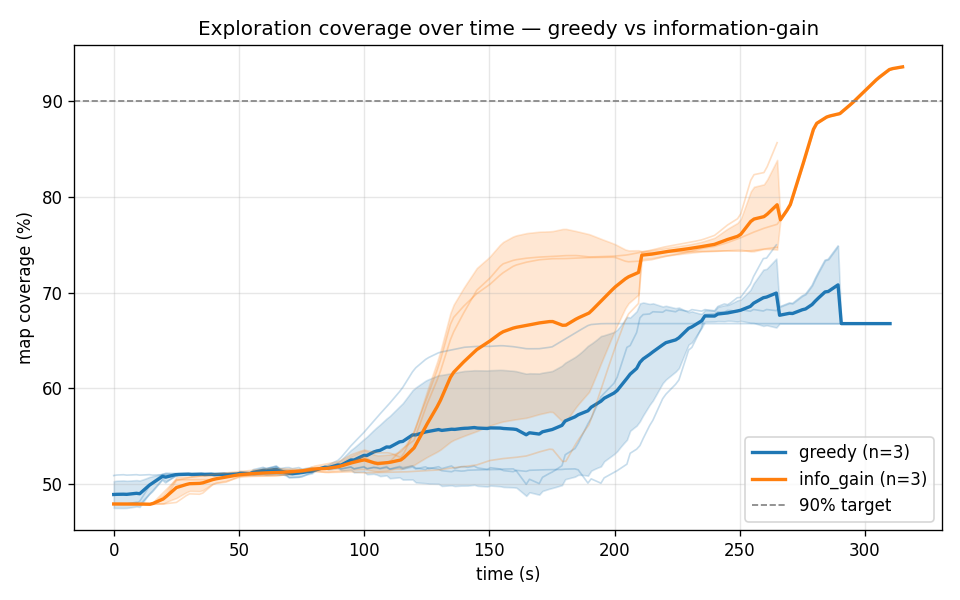
\includegraphics[width=0.62\linewidth]{coverage_over_time}\\[1.5mm]
  {\footnotesize\color{nccblue} Benchmark $n{=}3$ : le \textbf{gain d'information} (orange) atteint la cible
  90\,\% ; le \textbf{glouton} (bleu) plafonne $\sim$67--70\,\% sans jamais l'atteindre - il s'engage à
  ouvrir des pièces entières (plus d'inconnu par mètre), là où le glouton grignote localement et s'essouffle.}
\end{frame}

% -- Results 2 --
\begin{frame}{Résultats - couverture, carte et conformité}
  \begin{columns}[c]
  \begin{column}{0.5\linewidth}\centering
  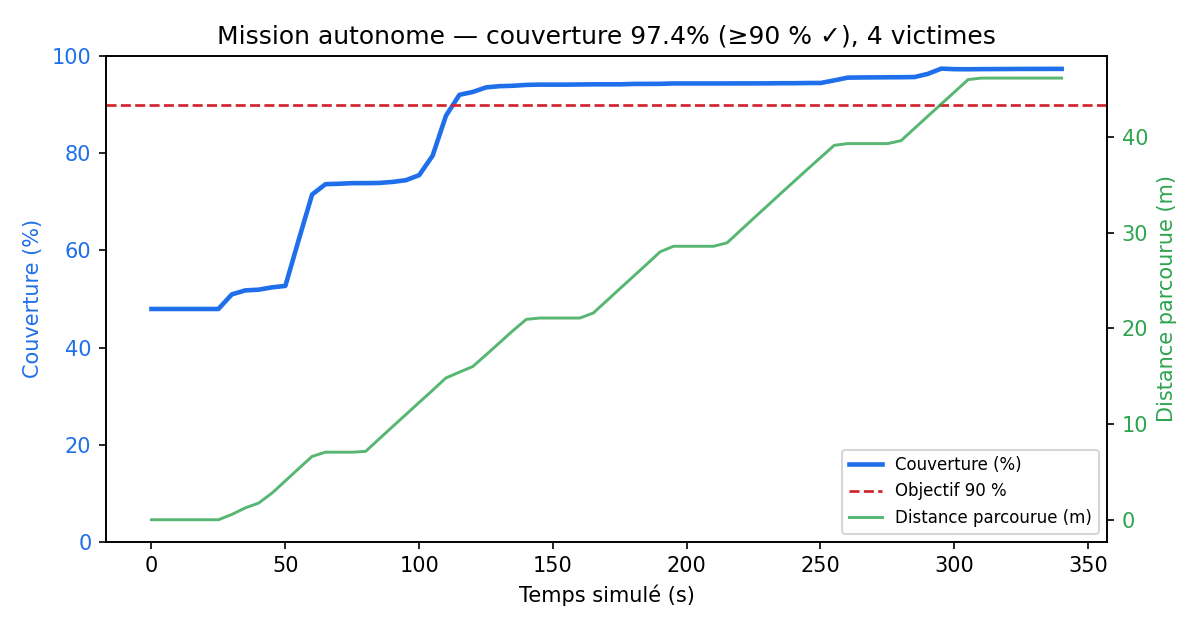
\includegraphics[width=0.96\linewidth]{coverage_curve}\\{\scriptsize Couverture \& chemin en fonction du temps, cible 90\,\%.}
  \end{column}
  \begin{column}{0.5\linewidth}\centering
  
\includegraphics[width=0.72\linewidth]{mission_map}\\{\scriptsize Carte finale : 4 victimes + tournée d'inspection autonome.}
  \end{column}
  \end{columns}
  \smallskip
  {\footnotesize\color{nccblue}\centering \textbf{97,35\,\% de couverture $\cdot$ 4/4 victimes $\cdot$ carte annotée $\cdot$ trajectoire enregistrée} - un clic, entièrement autonome.}
\end{frame}

% -- Team / git --
\begin{frame}{Équipe et collaboration}
  \begin{columns}[T]
  \begin{column}{0.52\linewidth}
  \footnotesize
  Branches \texttt{dev/*} par membre fusionnées dans \texttt{dev/bl} (intégration) :
  \begin{itemize}
    \item \textbf{Yimou} - exploration, SLAM/Nav2, cœur de perception
    \item \textbf{Julien} - décision BT, infra (WSL/GPU/RTF), résultats, intégration
    \item \textbf{Hugo} - monde / arène / cibles AprilTag
    \item \textbf{Paul} - support perception/détection, tests
  \end{itemize}
  \end{column}
  \begin{column}{0.46\linewidth}\centering
  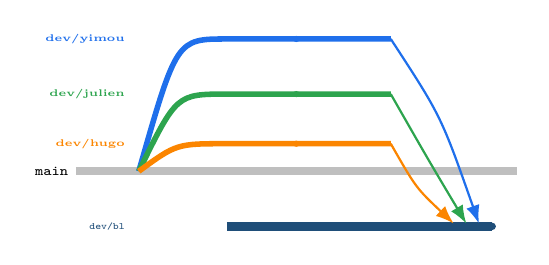
\begin{tikzpicture}[font=\scriptsize,xscale=0.8,yscale=0.7,transform shape]
    \draw[gray!50,line width=3pt] (0,0)--(7,0);\node[left] at (0,0){\texttt{main}};
    \foreach \y/\n/\c in {2.4/{dev/yimou}/nccsky,1.4/{dev/julien}/nccgreen,0.5/{dev/hugo}/nccorange}{
      \draw[\c,line width=2pt] (1,0) .. controls (1.6,\y) .. (2.4,\y) -- (5,\y);
      \node[\c,left,font=\tiny\bfseries] at (0.9,\y){\n};
      \fill[\c] (3.5,\y) circle (1.6pt);}
    \draw[nccblue,line width=3pt] (2.4,-1.0)--(6.6,-1.0);\node[nccblue,left,font=\tiny\bfseries] at (0.9,-1.0){\texttt{dev/bl}};
    \draw[-{Latex},nccsky,thick] (5,2.4) .. controls (5.8,1) .. (6.4,-0.95);
    \draw[-{Latex},nccgreen,thick] (5,1.4) .. controls (5.6,0.2) .. (6.2,-0.95);
    \draw[-{Latex},nccorange,thick] (5,0.5) .. controls (5.4,-0.3) .. (6.0,-0.95);
    \fill[nccblue] (6.6,-1.0) circle (2pt);
  \end{tikzpicture}\\
  {\scriptsize Trois axes de travail vers l'intégration \texttt{bl}.}
  \end{column}
  \end{columns}
\end{frame}

% -- Lessons --
\begin{frame}{Leçons apprises}
  \begin{itemize}
    \item \textbf{Mesurer avant de prescrire} - les causes « évidentes » (mémoire, Windows Update) étaient fausses deux fois ; les journaux d'événements ont trouvé les vraies (TDR GPU, une caméra affamée).
    \item \textbf{Un correctif en révèle un autre} - la détection de victimes a traversé six causes empilées.
    \item \textbf{Robuste l'emporte sur rigide} - exploration adaptative + balayage 360$^\circ$ ; et l'inspecteur récupère une pose qu'une autre machine n'atteint pas (attendre le costmap, se rabattre dans la pièce) - \emph{robustesse inter-machines}.
    \item \textbf{Conformité par conception} - un BT qui \emph{orchestre} (pas seulement supervise) respecte l'énoncé dans l'esprit, pas seulement à la lettre.
  \end{itemize}
  \vfill
  {\footnotesize\color{nccblue}Chronologie : L13 lancement $\cdot$ L14 architecture $\cdot$ L15 nœuds/SLAM $\cdot$ L16 BT+perception $\cdot$ L17 intégration/benchmark $\cdot$ L18 deux phases, run final, rapport.}
\end{frame}

% -- Thanks --
\begin{frame}[plain]
  \centering
  \vfill
  {\Large\color{nccblue}\textbf{Merci - Questions ?}}\\[10pt]
  {\small Nous remercions chaleureusement \textbf{Zhi Yan}, enseignant-chercheur à l'ENSTA,\\ pour le cours IA712 et son accompagnement.}\\[14pt]
  {\footnotesize \texttt{https://github.com/YiZeems/autonomous-search-and-rescue}}\\[4pt]
  {\scriptsize Julien GIMENEZ $\cdot$ Hugo FANCHINI $\cdot$ Paul CINTRA $\cdot$ Yimou ZHANG}
  \vfill
\end{frame}

\end{document}
